\section{Analisis Kondisi Saat Ini}
\label{sec:analisis-kondisi-saat-ini}

Subbab ini akan membahas tentang kondisi sistem yang ada saat ini. Penulis akan mengidentifikasi masalah yang ada sekarang dan menggambarkan kondisi sistem saat ini pada \autoref{fig:current-state}. Dengan memahami bagaimana sistem saat ini beroperasi dan mengidentifikasi keterbatasan yang ada, penulis dapat menentukan kebutuhan fungsional dan non-fungsional yang diperlukan untuk sistem yang akan dikembangkan.

% \begin{figure}[htbp]
%     \centering
%     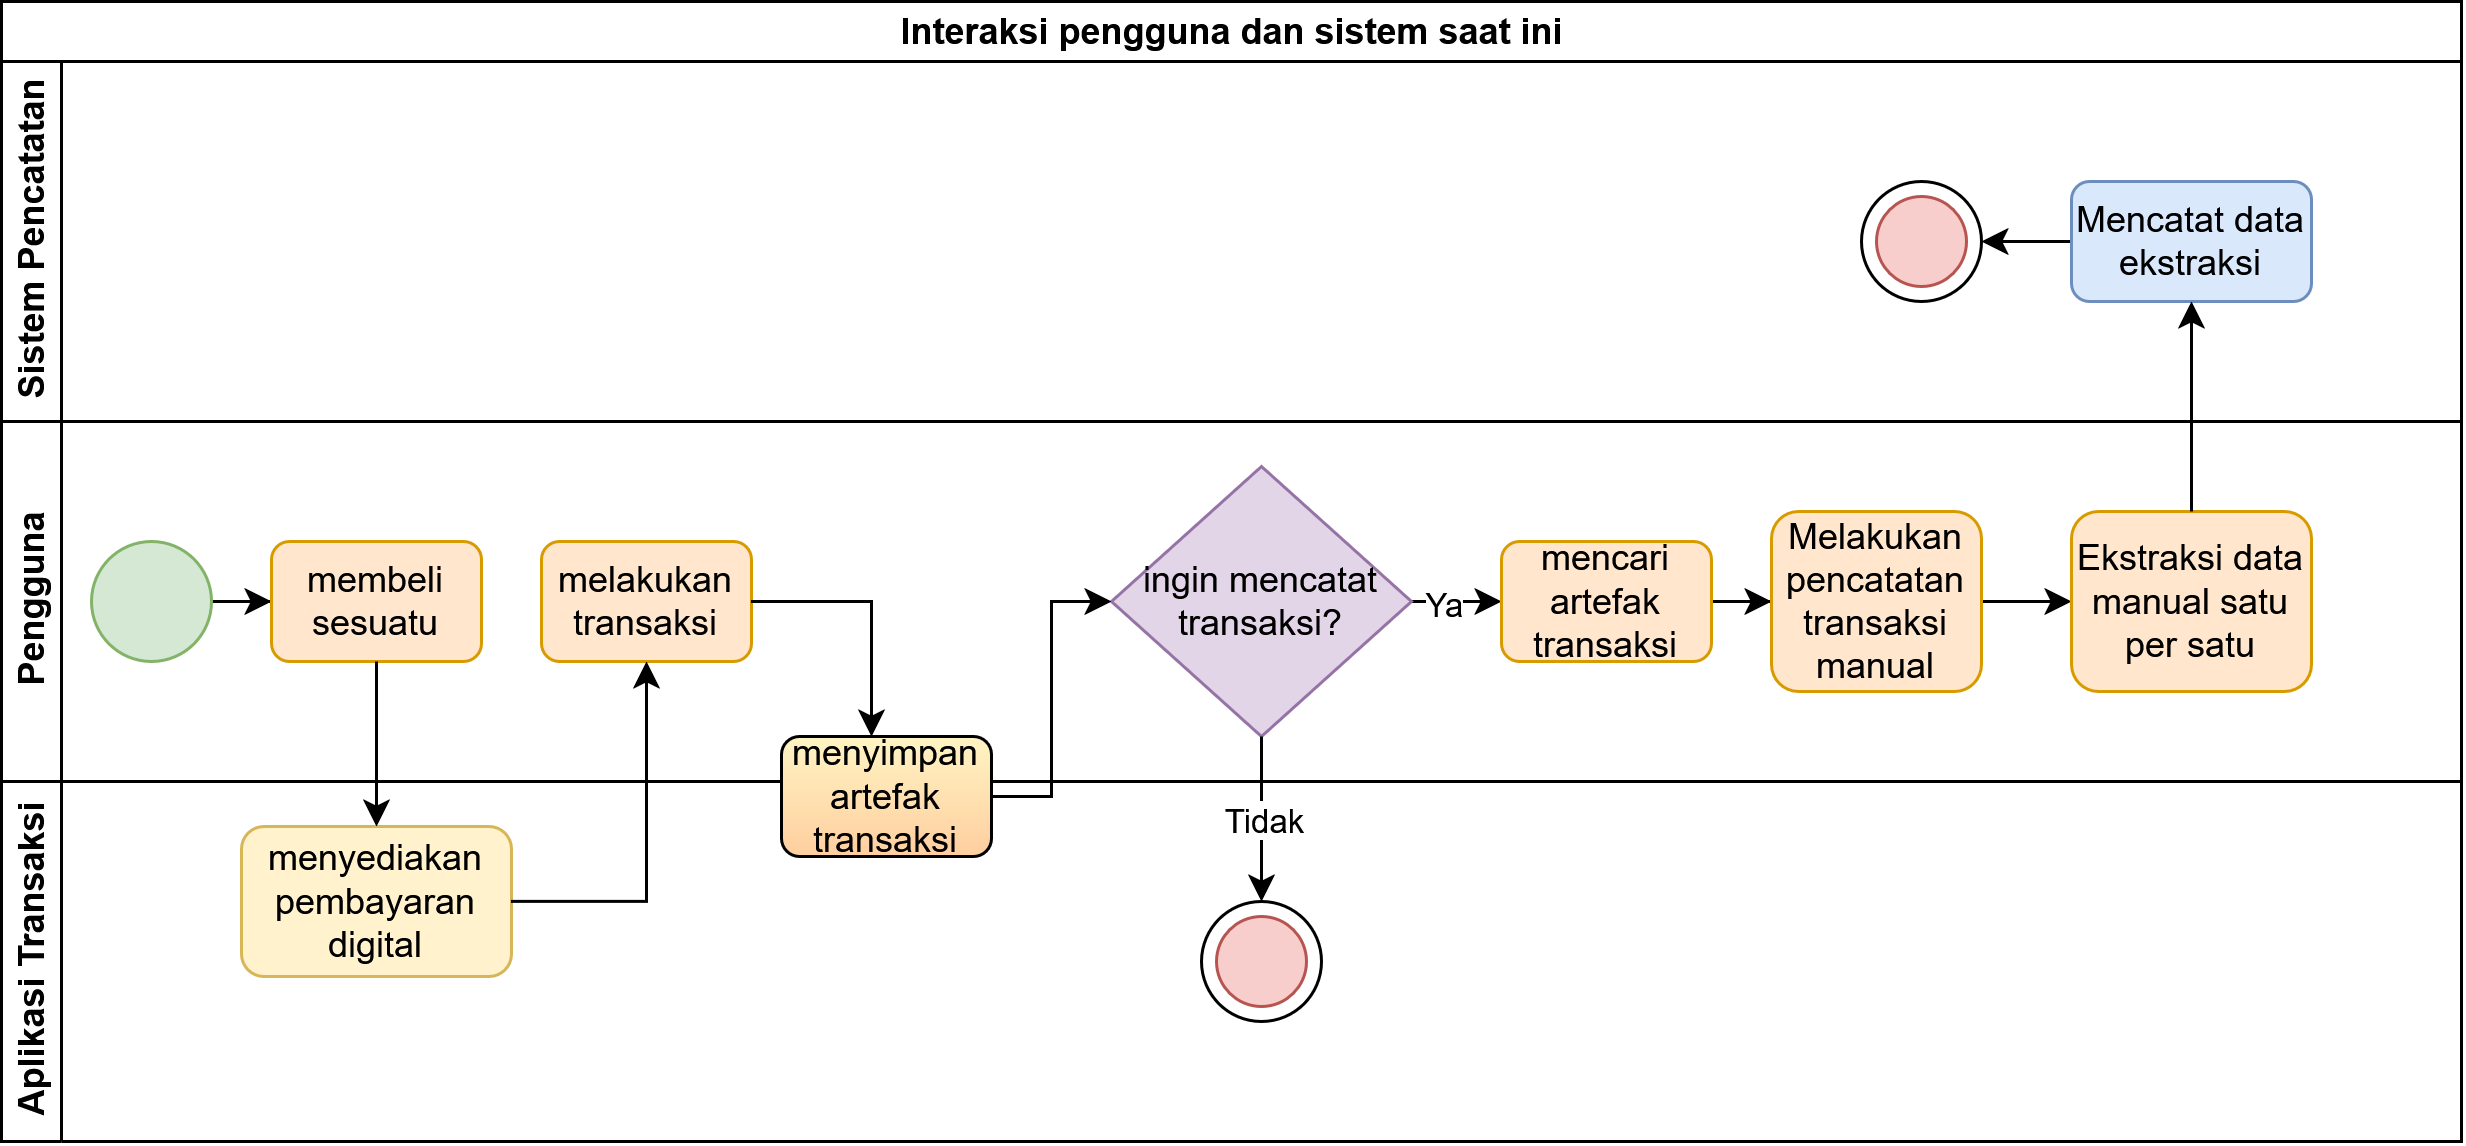
\includegraphics[width=0.8\textwidth]{images/current-state.png}
%     \caption{Kondisi sistem saat ini}
%     \label{fig:current-state}
% \end{figure}

